\documentclass{article}

\usepackage{arxiv}

\usepackage[utf8]{inputenc} % allow utf-8 input
\usepackage[T1]{fontenc}    % use 8-bit T1 fonts
\usepackage{lmodern}        % https://github.com/rstudio/rticles/issues/343
\usepackage{hyperref}       % hyperlinks
\usepackage{url}            % simple URL typesetting
\usepackage{booktabs}       % professional-quality tables
\usepackage{amsfonts}       % blackboard math symbols
\usepackage{nicefrac}       % compact symbols for 1/2, etc.
\usepackage{microtype}      % microtypography
\usepackage{graphicx}

\title{Stability of ecological and epidemiological models via
representation as Generalized Lotka-Volterra dynamics}

\author{
    Stefano Allesina
    \thanks{stefanoallesina.github.io}
   \\
    Department of Ecology \& Evolution \\
    University of Chicago \\
  Chicago, IL 60637 USA \\
  \texttt{\href{mailto:sallesina@uchicago.edu}{\nolinkurl{sallesina@uchicago.edu}}} \\
   \And
    Zachary R. Miller
   \\
    Department of Ecology \& Evolution \\
    University of Chicago \\
   \\
  \texttt{\href{mailto:zachmiller@uchicago.edu}{\nolinkurl{zachmiller@uchicago.edu}}} \\
  }

\usepackage{color}
\usepackage{fancyvrb}
\newcommand{\VerbBar}{|}
\newcommand{\VERB}{\Verb[commandchars=\\\{\}]}
\DefineVerbatimEnvironment{Highlighting}{Verbatim}{commandchars=\\\{\}}
% Add ',fontsize=\small' for more characters per line
\usepackage{framed}
\definecolor{shadecolor}{RGB}{248,248,248}
\newenvironment{Shaded}{\begin{snugshade}}{\end{snugshade}}
\newcommand{\AlertTok}[1]{\textcolor[rgb]{0.94,0.16,0.16}{#1}}
\newcommand{\AnnotationTok}[1]{\textcolor[rgb]{0.56,0.35,0.01}{\textbf{\textit{#1}}}}
\newcommand{\AttributeTok}[1]{\textcolor[rgb]{0.77,0.63,0.00}{#1}}
\newcommand{\BaseNTok}[1]{\textcolor[rgb]{0.00,0.00,0.81}{#1}}
\newcommand{\BuiltInTok}[1]{#1}
\newcommand{\CharTok}[1]{\textcolor[rgb]{0.31,0.60,0.02}{#1}}
\newcommand{\CommentTok}[1]{\textcolor[rgb]{0.56,0.35,0.01}{\textit{#1}}}
\newcommand{\CommentVarTok}[1]{\textcolor[rgb]{0.56,0.35,0.01}{\textbf{\textit{#1}}}}
\newcommand{\ConstantTok}[1]{\textcolor[rgb]{0.00,0.00,0.00}{#1}}
\newcommand{\ControlFlowTok}[1]{\textcolor[rgb]{0.13,0.29,0.53}{\textbf{#1}}}
\newcommand{\DataTypeTok}[1]{\textcolor[rgb]{0.13,0.29,0.53}{#1}}
\newcommand{\DecValTok}[1]{\textcolor[rgb]{0.00,0.00,0.81}{#1}}
\newcommand{\DocumentationTok}[1]{\textcolor[rgb]{0.56,0.35,0.01}{\textbf{\textit{#1}}}}
\newcommand{\ErrorTok}[1]{\textcolor[rgb]{0.64,0.00,0.00}{\textbf{#1}}}
\newcommand{\ExtensionTok}[1]{#1}
\newcommand{\FloatTok}[1]{\textcolor[rgb]{0.00,0.00,0.81}{#1}}
\newcommand{\FunctionTok}[1]{\textcolor[rgb]{0.00,0.00,0.00}{#1}}
\newcommand{\ImportTok}[1]{#1}
\newcommand{\InformationTok}[1]{\textcolor[rgb]{0.56,0.35,0.01}{\textbf{\textit{#1}}}}
\newcommand{\KeywordTok}[1]{\textcolor[rgb]{0.13,0.29,0.53}{\textbf{#1}}}
\newcommand{\NormalTok}[1]{#1}
\newcommand{\OperatorTok}[1]{\textcolor[rgb]{0.81,0.36,0.00}{\textbf{#1}}}
\newcommand{\OtherTok}[1]{\textcolor[rgb]{0.56,0.35,0.01}{#1}}
\newcommand{\PreprocessorTok}[1]{\textcolor[rgb]{0.56,0.35,0.01}{\textit{#1}}}
\newcommand{\RegionMarkerTok}[1]{#1}
\newcommand{\SpecialCharTok}[1]{\textcolor[rgb]{0.00,0.00,0.00}{#1}}
\newcommand{\SpecialStringTok}[1]{\textcolor[rgb]{0.31,0.60,0.02}{#1}}
\newcommand{\StringTok}[1]{\textcolor[rgb]{0.31,0.60,0.02}{#1}}
\newcommand{\VariableTok}[1]{\textcolor[rgb]{0.00,0.00,0.00}{#1}}
\newcommand{\VerbatimStringTok}[1]{\textcolor[rgb]{0.31,0.60,0.02}{#1}}
\newcommand{\WarningTok}[1]{\textcolor[rgb]{0.56,0.35,0.01}{\textbf{\textit{#1}}}}

\usepackage{longtable,booktabs,array}
\usepackage{calc} % for calculating minipage widths
% Correct order of tables after \paragraph or \subparagraph
\usepackage{etoolbox}
\makeatletter
\patchcmd\longtable{\par}{\if@noskipsec\mbox{}\fi\par}{}{}
\makeatother
% Allow footnotes in longtable head/foot
\IfFileExists{footnotehyper.sty}{\usepackage{footnotehyper}}{\usepackage{footnote}}
\makesavenoteenv{longtable}

% Pandoc citation processing
\newlength{\csllabelwidth}
\setlength{\csllabelwidth}{3em}
\newlength{\cslhangindent}
\setlength{\cslhangindent}{1.5em}
% for Pandoc 2.8 to 2.10.1
\newenvironment{cslreferences}%
  {}%
  {\par}
% For Pandoc 2.11+
\newenvironment{CSLReferences}[2] % #1 hanging-ident, #2 entry spacing
 {% don't indent paragraphs
  \setlength{\parindent}{0pt}
  % turn on hanging indent if param 1 is 1
  \ifodd #1 \everypar{\setlength{\hangindent}{\cslhangindent}}\ignorespaces\fi
  % set entry spacing
  \ifnum #2 > 0
  \setlength{\parskip}{#2\baselineskip}
  \fi
 }%
 {}
\usepackage{calc} % for calculating minipage widths
\newcommand{\CSLBlock}[1]{#1\hfill\break}
\newcommand{\CSLLeftMargin}[1]{\parbox[t]{\csllabelwidth}{#1}}
\newcommand{\CSLRightInline}[1]{\parbox[t]{\linewidth - \csllabelwidth}{#1}\break}
\newcommand{\CSLIndent}[1]{\hspace{\cslhangindent}#1}

\usepackage{amsmath}
\usepackage{xcolor}


\begin{document}
\maketitle

\def\tightlist{}


\begin{abstract}
Enter the text of your abstract here.
\end{abstract}

\keywords{
    Lotka-Volterra
   \and
    Stability
   \and
    Quasi-polynomial
   \and
    Lyapunov function
  }

\hypertarget{introduction}{%
\section{Introduction}\label{introduction}}

Blah, blah

\hypertarget{generalized-lotka-volterra-model}{%
\section{Generalized Lotka-Volterra
model}\label{generalized-lotka-volterra-model}}

\label{sec:glv}

\begin{equation}
\label{eq:glv}
\dot{x}_i = x_i \left(r_i + \sum_{j=1}^m A_{ij} x_j \right)
\end{equation}

\hypertarget{quasi-polynomial-systems}{%
\section{Quasi-Polynomial systems}\label{quasi-polynomial-systems}}

\label{sec:qp}

\begin{equation}
\label{eq:qp}
\dot{y}_i = y_i \left( \lambda_i + \sum_{j = 1}^m M_{ij} \prod_{k = 1}^n y_k^{B_{jk}} \right)
\end{equation}

where \(\lambda\) is a vector of length \(n\); \(M\) is a matrix of size
\(n \times m\) containing real coefficients, and \(B\) a matrix of size
\(m \times n\), also containing real coefficients. If \(n = m\), and
thus \(M\) is a square matrix, and \(B=I_n\) the model reduces to the
Generalized Lotka-Volterra model in Eq. \ref{eq:glv} with
\(r = \lambda\) and \(A = M\). If \(B\) contains only integers, Eq.
\ref{eq:qp} defines a \emph{polynomial} system of differential
equations; relaxing this condition to admit \(B\) composed of real
numbers, we obtain a \emph{quasi-polynomial} (QP) system.

\begin{center}\rule{0.5\linewidth}{0.5pt}\end{center}

\textbf{QP-representation of Leslie-Gower predator-prey model}

\begin{equation}
\label{eq:lg}
\begin{cases}
\dot{y}_1 = y_1 (\rho_1 - y_1- \alpha_1 y_2)\\
\dot{y}_2 = y_2 \left(\rho_2 - \alpha_2 \frac{y_2}{y_1} \right)
\end{cases}
\end{equation}

with \(y_1\) being the prey, \(y_2\) the predator, and all coefficients
positive. The system differs from GLV in that we have a ratio between
the predator and prey in the equation for the predator. The system is
however in QP form, as seen by defining:

\begin{equation}
\label{eq:lgqp}
\lambda = \begin{pmatrix}
\rho_1\\
\rho_2
\end{pmatrix} \quad 
M = \begin{pmatrix}
-1 & -\alpha_1 & 0\\
0 & 0 & -\alpha_2
\end{pmatrix} \quad
B = \begin{pmatrix}
1 & 0 \\
0 & 1 \\
1 & -1
\end{pmatrix}
\end{equation}

\begin{center}\rule{0.5\linewidth}{0.5pt}\end{center}

\hypertarget{from-quasi-polynomial-to-generalized-lotka-volterra}{%
\section{From Quasi-Polynomial to Generalized
Lotka-Volterra}\label{from-quasi-polynomial-to-generalized-lotka-volterra}}

\label{sec:qptoglv}

We define a set of \(m\) \emph{quasi-monomials}:

\begin{equation}
\label{eq:quasimono}
x_j = \prod_{k=1}^n y_k^{B_{jk}}
\end{equation}

\begin{center}\rule{0.5\linewidth}{0.5pt}\end{center}

\textbf{Quasi-monomials for the Leslie-Gower model}

For the Leslie-Gower model in Eq. \ref{eq:lg} we identify three
quasi-monomials:

\begin{equation}
\label{eq:lgqm}
\begin{cases}
x_1 = y_1^1 \, y_2^0 = y_1\\
x_2 = y_1^0 \, y_2^1 = y_2\\
x_3 = y_1^{-1} \, y_2^1 = \frac{y_2}{y_1}
\end{cases}
\end{equation}

\begin{center}\rule{0.5\linewidth}{0.5pt}\end{center}

By chain rule, we have:

\begin{equation}
\label{eq:quasimonodt}
\begin{aligned}
\dot{x}_j &= \sum_k B_{jk}\, \dot{y}_k \, y_{k}^{(B_{jk} -1)} \prod_{l \neq k} y_{l}^{B_{jl}}\\
&=\sum_k B_{jk}\, \frac{\dot{y}_k}{y_k} \prod_{l} y_{l}^{B_{jl}}\\
&=\sum_k B_{jk}\, \frac{\dot{y}_k}{y_k} x_j\\
&=x_j \sum_k B_{jk}\, \frac{\dot{y}_k}{y_k} \\
&=x_j \left(\sum_k B_{jk} \lambda_k + \sum_k B_{jk} \sum_l M_{kl} \prod_l y_l^{B_{kl}} \right)\\
&=x_j \left(\sum_k B_{jk} \lambda_k + \sum_k B_{jk} \sum_l M_{kl} x_l \right)\\
&=x_j \left((B \lambda)_j + \sum_l (B M)_{jl} x_l \right)\\
&=x_j \left(r_j + \sum_l A_{jl} x_l \right)
\end{aligned}
\end{equation}

where we have defined \(A = BM\) and \(r = B \lambda\), \((B\lambda)_j\)
is the \(j^{\text{th}}\) element of the vector \(B\lambda\) and
\((B M)_{jl}\) is the coefficient in row \(j\) and column \(l\) of the
matrix \(BM\).

Via the quasi-monomial transformation in Eq. \ref{eq:quasimono} we have
turned the \(n-\)dimensional QP-system in Eq. \ref{eq:qp} into an
\(m-\)dimensional GLV system in Eq. \ref{eq:glv}.

\begin{center}\rule{0.5\linewidth}{0.5pt}\end{center}

\textbf{GLV representation of the Leslie-Gower model}

We can represent the Leslie-Gower model in Eq. \ref{eq:lg} as a
three-dimensional GLV model defined by the quasi-monomials in Eq.
\ref{eq:lgqm} and:

\begin{equation}
r = B \lambda = \begin{pmatrix}
\rho_1\\
\rho_2\\
\rho_2 - \rho_1
\end{pmatrix}
\quad
A = B M = \begin{pmatrix}
-1 & -\alpha_1 & 0\\
0 & 0 & -\alpha_2\\
1 & \alpha_1 & -\alpha_2
\end{pmatrix}
\end{equation}

Note that \(A\) is rank deficient, given that the third row can be
written as the difference between the second and first row.
Rank-deficiency of \(A\) is expected whenever \(m > n\) (as here, where
we went from two to three equations).

\begin{center}\rule{0.5\linewidth}{0.5pt}\end{center}

\hypertarget{examples-of-citations-figures-tables-references}{%
\section{Examples of citations, figures, tables,
references}\label{examples-of-citations-figures-tables-references}}

\label{sec:others}

You can insert references. Here is some text (Kour and Saabne 2014b,
2014a) and see Hadash et al. (2018).

The documentation for \verb+natbib+ may be found at

You can use custom blocks with LaTeX support from \textbf{rmarkdown} to
create environment.

\begin{center}
\url{http://mirrors.ctan.org/macros/latex/contrib/natbib/natnotes.pdf\%7D}

\end{center}

Of note is the command \verb+\citet+, which produces citations
appropriate for use in inline text.

You can insert LaTeX environment directly too.

\begin{verbatim}
   \citet{hasselmo} investigated\dots
\end{verbatim}

produces

\begin{quote}
  Hasselmo, et al.\ (1995) investigated\dots
\end{quote}

\begin{center}
  \url{https://www.ctan.org/pkg/booktabs}
\end{center}

\hypertarget{figures}{%
\subsection{Figures}\label{figures}}

You can insert figure using LaTeX directly.

See Figure \ref{fig:fig1}. Here is how you add footnotes. {[}\^{}Sample
of the first footnote.{]}

\begin{figure}
  \centering
  \fbox{\rule[-.5cm]{4cm}{4cm} \rule[-.5cm]{4cm}{0cm}}
  \caption{Sample figure caption.}
  \label{fig:fig1}
\end{figure}

But you can also do that using R.

\begin{Shaded}
\begin{Highlighting}[]
\FunctionTok{plot}\NormalTok{(mtcars}\SpecialCharTok{$}\NormalTok{mpg)}
\end{Highlighting}
\end{Shaded}

\begin{figure}
\centering
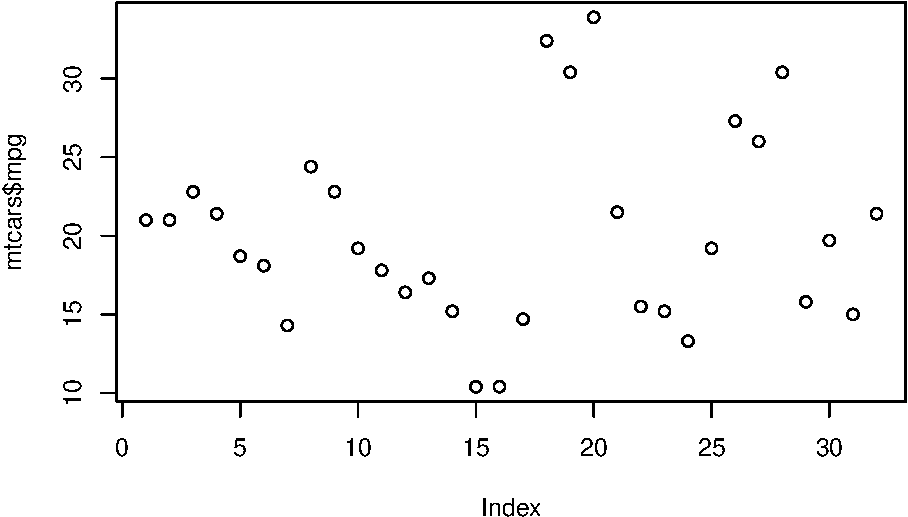
\includegraphics{GLV_embedding_files/figure-latex/fig2-1.pdf}
\caption{Another sample figure}
\end{figure}

You can use \textbf{bookdown} to allow references for Tables and
Figures.

\hypertarget{tables}{%
\subsection{Tables}\label{tables}}

Below we can see how to use tables.

See awesome Table\textasciitilde{}\ref{tab:table} which is written
directly in LaTeX in source Rmd file.

\begin{table}
 \caption{Sample table title}
  \centering
  \begin{tabular}{lll}
    \toprule
    \multicolumn{2}{c}{Part}                   \\
    \cmidrule(r){1-2}
    Name     & Description     & Size ($\mu$m) \\
    \midrule
    Dendrite & Input terminal  & $\sim$100     \\
    Axon     & Output terminal & $\sim$10      \\
    Soma     & Cell body       & up to $10^6$  \\
    \bottomrule
  \end{tabular}
  \label{tab:table}
\end{table}

You can also use R code for that.

\begin{Shaded}
\begin{Highlighting}[]
\NormalTok{knitr}\SpecialCharTok{::}\FunctionTok{kable}\NormalTok{(}\FunctionTok{head}\NormalTok{(mtcars), }\AttributeTok{caption =} \StringTok{"Head of mtcars table"}\NormalTok{)}
\end{Highlighting}
\end{Shaded}

\begin{longtable}[]{@{}lrrrrrrrrrrr@{}}
\caption{Head of mtcars table}\tabularnewline
\toprule
& mpg & cyl & disp & hp & drat & wt & qsec & vs & am & gear & carb \\
\midrule
\endfirsthead
\toprule
& mpg & cyl & disp & hp & drat & wt & qsec & vs & am & gear & carb \\
\midrule
\endhead
Mazda RX4 & 21.0 & 6 & 160 & 110 & 3.90 & 2.620 & 16.46 & 0 & 1 & 4 &
4 \\
Mazda RX4 Wag & 21.0 & 6 & 160 & 110 & 3.90 & 2.875 & 17.02 & 0 & 1 & 4
& 4 \\
Datsun 710 & 22.8 & 4 & 108 & 93 & 3.85 & 2.320 & 18.61 & 1 & 1 & 4 &
1 \\
Hornet 4 Drive & 21.4 & 6 & 258 & 110 & 3.08 & 3.215 & 19.44 & 1 & 0 & 3
& 1 \\
Hornet Sportabout & 18.7 & 8 & 360 & 175 & 3.15 & 3.440 & 17.02 & 0 & 0
& 3 & 2 \\
Valiant & 18.1 & 6 & 225 & 105 & 2.76 & 3.460 & 20.22 & 1 & 0 & 3 & 1 \\
\bottomrule
\end{longtable}

\hypertarget{lists}{%
\subsection{Lists}\label{lists}}

\begin{itemize}
\tightlist
\item
  Item 1
\item
  Item 2
\item
  Item 3
\end{itemize}

\hypertarget{refs}{}
\begin{CSLReferences}{1}{0}
\leavevmode\hypertarget{ref-hadash2018estimate}{}%
Hadash, Guy, Einat Kermany, Boaz Carmeli, Ofer Lavi, George Kour, and
Alon Jacovi. 2018. {``Estimate and Replace: A Novel Approach to
Integrating Deep Neural Networks with Existing Applications.''}
\emph{arXiv Preprint arXiv:1804.09028}.

\leavevmode\hypertarget{ref-kour2014fast}{}%
Kour, George, and Raid Saabne. 2014a. {``Fast Classification of
Handwritten on-Line Arabic Characters.''} In \emph{Soft Computing and
Pattern Recognition (SoCPaR), 2014 6th International Conference of},
312--18. IEEE.

\leavevmode\hypertarget{ref-kour2014real}{}%
---------. 2014b. {``Real-Time Segmentation of on-Line Handwritten
Arabic Script.''} In \emph{Frontiers in Handwriting Recognition (ICFHR),
2014 14th International Conference on}, 417--22. IEEE.

\end{CSLReferences}

\bibliographystyle{unsrt}
\bibliography{references.bib}


\end{document}
